\documentclass[a4paper,10pt]{article}
\usepackage[utf8]{inputenc}
\usepackage[english,russian]{babel}
\usepackage[top=2cm,bottom=3cm,left=2cm,right=2cm,nohead]{geometry}
\usepackage{multicol}
\usepackage{graphicx}

\graphicspath{{images/}}


\begin{document}
\section*{задачи многомодульное программирование}
\begin{enumerate}
    
    \item ЕСЛИ вы не открывали пример многомодульного программирования откройте - можно на виртуалке всех команды в readme файлике после возвращайтесь!
    \item Синтаксис и Семантика public extrn\par
Синтаксис: public имя {, имя} \\
Семантика: ассемблер сохраняет информацию об этих именах в объектом модуле, делая её доступной для линковщика \par
Синтаксис: extrn имя:тип {, имя:тип} \\
Семантика: Ассемблер испольует информацию об именах и их типе для и обозначает что в модуле их нет и сообщает об этом в объектном файле, если имя присутствует то сделает имя public \par
    \item Будет ли ошибка?
\begin{verbatim}
include console.inc

.code
myuniquestart: 
    outstrln 'HelloWorld'
    exit
end myuniquestart
\end{verbatim}\par нет не будет
    \item Вопрос со звёздочкой: будет ли ошибка?
\begin{verbatim}
include console.inc

.code
start: 
    outstrln 'HelloWorld'
    exit
end
\end{verbatim}
    Если да то опишите как исправить (не приписывая после end start) \par
    будет не задана точка входа линковщик не знает где стартовать для исправления необходимо указать ключ /Entry:\_start (причём \_ добавится так как .console.inc есть прописан stdcall)
    \item ml /c /coff /Fl main.asm - стандартная компиляция object файла для нас (или через wine) поясните за каждый ключ \\
    \begin{tabular*}{15cm}{c|c}
        \hline
        /c &  только компиляция \\
        \hline
        /coff & требуемый тип объектного файла \\
        \hline
        /Fl & просит компилятор создать листинг (отчёт о компиляции)\\
        \hline
    \end{tabular*}
    \item опишите что случится с секциями .code разных модулей после линковки в 1 загружаемый файл.
Секции .code сольются в одну секцию, все смещения будут подставлены\\
    \item MyProc proto :byte,:dword,:byte - для чего существует возможность описывать прототип опишите ситуацию \\
proto может понадобится для удобства при импорте из другого модуля если нам известно соглашение то ассемблер сам переменует согласно нему и этим параметрам, а мы и дальше сможем использовать MyProc а не \_MyProc@12 при написании кода \\
    \item private для чего существует \\
по умолчанию в ассемблере все процедуры - публичные, private явно укажет что процедура может использоваться только в этом модуле
    \item найдите все ошибки исправьте после линковки и запуска должен отработать next\_day взяв параметры как у прототипа
\begin{verbatim}
.686; доп модуль
.XMM

.model flat, stdcall
public next_day@12
.code
; рпринимает 3 параметра
next_day@12:
next_day proc private
push ebp
mov ebp, esp
...
pop ebp
ret 12
next_day endp
end
\end{verbatim}


\begin{verbatim}
.686; основной модуль
.XMM

.model flat

.data 
op1 db ?
op2 dd ?
op3 db ?
.code
Start:
    next_day proto :byte,:dword,:byte
    push op3
    push op2
    push op1
    call next_day
    ...
end Start
\end{verbatim}
необходимо исправить .model flat, stdcall
\newpage
    \item схематично стрелками как на лекции обрисуйте все выходы и входы сделайте вывод о линковке подпишите внешние имена в формате stdcall (указана опция: option proc:private)
\begin{multicols}{2}
\begin{verbatim}
;main.asm
public cringe, twop@4
.data
    extrn love:real4; 7F800000h))
    cringe dw ?
    
.code
twop@4:
twop proc
...
twop endp

onep proc public
...
onep endp
Start:
    ...
end Start
\end{verbatim}
\columnbreak
\begin{verbatim}
;module.asm
public love

.data
    love real4 ?
    extrn cringe:word
    extrn true:byte
    
twop proto :dword
.code
    extrn onep@0:proc
    ...
end
\end{verbatim}
\end{multicols}
пролог в обоих случая Стандартный\par
\begin{verbatim}
    .686
    
    .model flat, stdcall
    option proc:private
\end{verbatim}
\begin{figure}[htbp]
    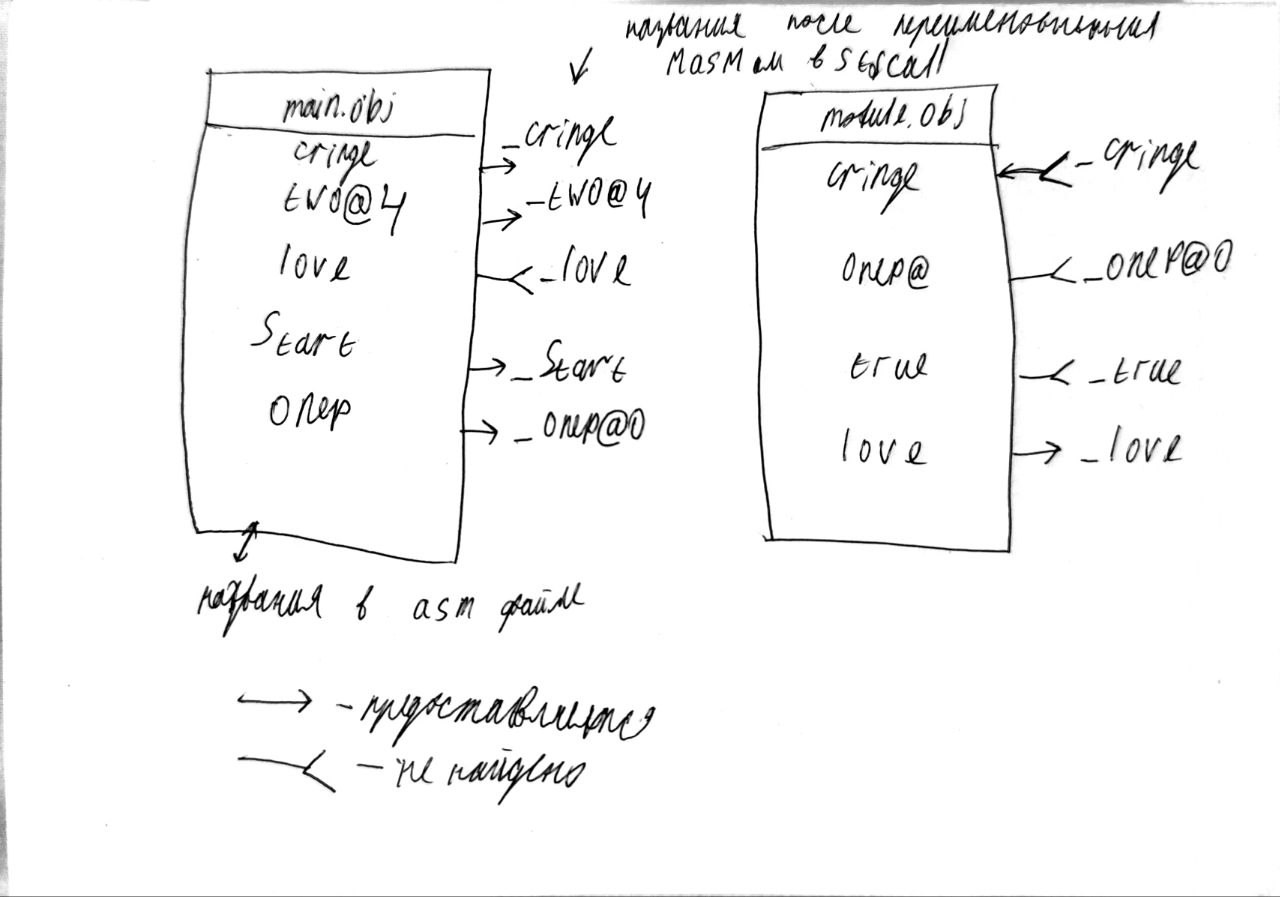
\includegraphics[width=0.85\textwidth]{мегасхема.png}
\end{figure}
\newpage
Проверим себя через утилиту nm
\begin{multicols}{2}
main.obj
\begin{verbatim}
001220fc a @comp.id
00000000 D _cringe
00000000 d .data
00000000 i .drectve
            U _love
00000002 T _onep@0
00000004 T _Start
00000000 t .text
00000000 t _twop@0
00000000 T _twop@4
\end{verbatim}
\columnbreak
module.obj
\begin{verbatim}
001220fc a @comp.id
            U _cringe
00000000 d .data
00000000 D _love
            U _onep@0
00000000 t .text
            U _true
\end{verbatim}
\end{multicols}

Если можно убрать ошибки совместимости вычеркиванием одной строки сделайте \\
да при линковке недостаёт одного момента 'true' вычеркнем правду( 
    \item дан листинг указать на месте подчёркиваний числа или буквы
\begin{multicols}{2}
\begin{verbatim}
00000000			.data
        extrn hapiness:byte
00000000  00000005 [		    garbage db 5 dup (?)
00
]
00000005 2A			    mydata db 42; 
\end{verbatim}
\columnbreak
\begin{verbatim}
    000000XX  88 25 ________ _	   mov hapiness, ah
    000000XX  C6 05 ________ _	   mov mydata, 8
    08
\end{verbatim}
\end{multicols} \par
первый пропуски - hapiness - переменная внешняя потому будет \textbf{00000000 E} (E - extern) так как мы не знаем где будет находится hapiness \\
второй пропуск - mydata обратимся к листингу слева секция .data смещение от начала 00000005 так как секции  будут сливаться и нам известно лишь смещение для данного объектного модуля то будет буква R итого \textbf{00000005 R}
\end{enumerate}

\end{document}